\documentclass[11pt,letterpaper]{article}
\usepackage[margin=0.8in]{geometry}
\usepackage[T1]{fontenc}
\usepackage{lmodern,microtype}
\usepackage{booktabs,tabularx,array,xcolor,tikz}
\usetikzlibrary{arrows.meta}
\usepackage{enumitem,fancyhdr,titlesec}
\usepackage[colorlinks=true,linkcolor=teal!65!black,urlcolor=teal!65!black,citecolor=teal!65!black]{hyperref}
\definecolor{ink}{HTML}{173447}
\definecolor{accent}{HTML}{147D83}
\definecolor{pale}{HTML}{EDF5F5}
\hypersetup{pdftitle={ComputerLM: Persistent State and Asynchronous Reasoning for Fast Computer Use},pdfauthor={J.D. Krasnick}}
\setlength{\parindent}{0pt}
\setlength{\parskip}{5pt}
\setlength{\emergencystretch}{2em}
\setlist[itemize]{leftmargin=1.25em,itemsep=3pt,topsep=3pt}
\setlist[enumerate]{leftmargin=1.45em,itemsep=4pt,topsep=3pt}
\titleformat{\section}{\large\bfseries\color{ink}}{\thesection}{0.6em}{}
\titleformat{\subsection}{\normalsize\bfseries\color{ink}}{\thesubsection}{0.6em}{}
\titlespacing*{\section}{0pt}{10pt}{5pt}
\titlespacing*{\subsection}{0pt}{7pt}{3pt}
\pagestyle{fancy}\fancyhf{}
\fancyhead[L]{\small\color{ink}ComputerLM}
\fancyhead[R]{\small Research proposal / Draft 0.9}
\fancyfoot[L]{\footnotesize J.D. Krasnick}
\fancyfoot[R]{\footnotesize\thepage}
\setlength{\headheight}{14pt}
\renewcommand{\headrulewidth}{0.3pt}
\begin{document}
\thispagestyle{empty}
{\small\bfseries\color{accent}RESEARCH PROPOSAL\hfill 10 NOVEMBER 2026}
\vspace{8pt}

{\LARGE\bfseries\color{ink}ComputerLM\par}
{\large Persistent State and Asynchronous Reasoning for Fast Computer Use\par}
\vspace{4pt}
J.D. Krasnick\hfill\href{https://github.com/JDKrasnick/computerlm}{github.com/JDKrasnick/computerlm}

\textbf{Summary.} ComputerLM combines a small recurrent controller with a deeper reasoning path that continues while the controller acts. Both observe the interface and maintain living task state. Slow reasoning communicates subgoals through learned latent vectors; fast control grounds them into actions and predicts short-term consequences. The objective is to match the strongest available GUI systems on easy and medium browser/desktop workflows, prioritizing faster completion and then lower cost. The integrated model remains untrained; these gains are hypotheses to test.

\section{Proposed architecture}
Many workflows contain a planning decision followed by routine interactions. ComputerLM aims to reuse that decision, carry progress forward, and overlap useful reasoning with execution and application delays.

\begin{figure}[h!]
\centering
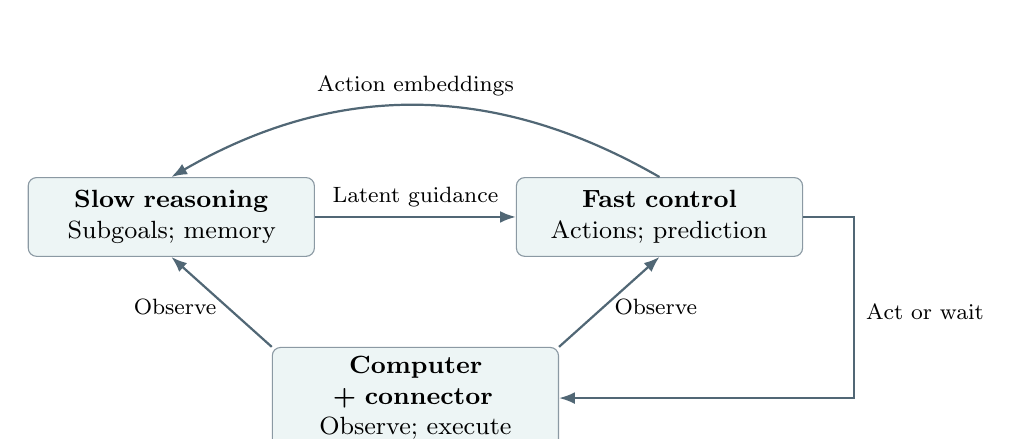
\begin{tikzpicture}[font=\small,box/.style={draw=ink!50,rounded corners=3pt,align=center,minimum height=10mm,text width=34mm,fill=pale},arr/.style={-{Latex[length=2mm]},thick,draw=ink!75}]
\node[box] (slow) at (0,2.3) {\textbf{Slow reasoning}\\Subgoals; memory};
\node[box] (fast) at (6.2,2.3) {\textbf{Fast control}\\Actions; prediction};
\node[box] (ui) at (3.1,0) {\textbf{Computer + connector}\\Observe; execute};
\draw[arr] (slow) -- node[above,font=\footnotesize]{Latent guidance} (fast);
\draw[arr] (fast.north) to[bend right=30] node[above,font=\footnotesize]{Action embeddings} (slow.north);
\draw[arr] (ui.north west) -- node[pos=.45,left,font=\footnotesize]{Observe} (slow.south);
\draw[arr] (ui.north east) -- node[pos=.45,right,font=\footnotesize]{Observe} (fast.south);
\draw[arr] (fast.east) -- ++(.65,0) |- (ui.east);
\node[anchor=west,font=\footnotesize] at (8.7,1.1) {Act or wait};
\end{tikzpicture}
\end{figure}

\textbf{Fast path.} A custom recurrent controller combines fresh visual features, action history, persistent state, and slow guidance. Only this path executes human-style GUI actions: clicking, typing, scrolling, dragging, keyboard shortcuts, or waits. The initial interface excludes shell, direct-file, DOM, and API shortcuts. Fast control predicts bounded action consequences; actual observations establish their effects.

\textbf{Slow path.} Adapt a suitably sized pretrained VLM into an input encoder, shared recurrent middle blocks, and guidance readout. It reasons continuously during an active task, including while fast control acts or waits. Guidance expresses dependencies such as \emph{find X to obtain Y} in latent space. A trained interface makes those vectors useful to the controller; slow reasoning cannot directly act on the computer. The checkpoint and size remain open.

\textbf{Perception and state.} Begin with native VLM screen encoding plus available accessibility/UI text. Cache identical encoder inputs under matching settings; fully encode changed screens. Recurrent state survives interactions and pause/resume, then resets between unrelated tasks. Preserve exact instructions, text payloads, action acknowledgements, and evidence references alongside compressed state. Action embeddings report operations and arguments; they do not represent every possible environment state.

\clearpage
\section{Design rationale and development}
Recurrent Memory Transformer carries learned memory between input segments~\cite{rmt}. Fast-in-Slow and DuoCore-FS provide robotics precedents for fast/slow cooperation and asynchronous latent guidance~\cite{fastinslow,duocore}. In GUI research, iSHIFT conditionally requests more visual processing after latent deliberation~\cite{ishift}; GUI-JEPA studies lightweight latent action scoring~\cite{guijepa}. These support components, not the complete architecture. Native VLM perception has a detailed precedent in Qwen2.5-VL~\cite{qwenvision}.

\textbf{Fresh evidence.} Screens become available to both paths immediately. Compare next-cycle intake with trained early/middle/late adapters, preserving state and measuring reaction delay and recovery. Initial episodes follow one instruction; later live steering can revise goal state through the slow update interface and propagate revised guidance.

\textbf{Adaptive execution.} A central ablation compares immediate highest-scoring action selection with learned deferral for additional fast computation or fresher slow guidance. Prediction supports this decision; a prediction-disabled control tests its separate contribution. Both variants retain continuous slow reasoning and ordinary waits for pending UI operations. Action probability alone is not assumed to measure correctness.

\textbf{Local constraints.} Prefer Apple-Silicon-class inference with compact models, bounded state, and realistic unified-memory use. Initially target one GPU with CPU support. Custom scheduling may be needed; profile fit, slow progress, and fast tail latency. Exact hardware and serving software remain open. Approximate visual reuse is optional future work.

\subsection{Staged training proposal}
Training hardware and compute/data budgets remain unspecified. Begin with a small diagnostic:
\begin{enumerate}
\item \textbf{Preserve pretrained capability.} Establish one-pass parity and stable recurrent adaptation. Initially retain native perception; select frozen weights, adapters, and recurrent depth from development evidence.
\item \textbf{Learn execution and guidance together.} Train the controller and latent interface on chronological screen--action--outcome sequences. Include persistent memory, exact text access, failed actions, recovery, and delayed or missing guidance.
\item \textbf{Add prediction and adaptive computation.} Supervise fast predictions with actual transitions; train and compare action/deferral policies. Collect learner failures for refinement, considering RL after useful supervised behaviour is established.
\end{enumerate}
Training uses only information available at each decision. Keep held-out outputs and corrections outside training. Memory across observations and repeated internal reasoning depth are separate: the latter adds computation even when no thinking text is generated.

\section{Evaluation objective}
Use a balanced browser/desktop suite with fixed easy/medium criteria. Select the strongest available GUI references before testing; retain same-backbone sequential and component controls. Match observations, GUI actions, and resets. Equalize hardware for local controls; disclose hosted-reference hardware and network differences. Measure complete trajectories rather than action latency alone~\cite{speedrun}.

\clearpage
\section{Evidence required and remaining decisions}
\textbf{Primary result: faster completion at matched accuracy.} Predeclare the acceptable accuracy difference, task mix, repetitions, and improvement thresholds before held-out testing. Verify exact task outcomes independently and report failed attempts. Include timing on jointly solved tasks without dropping other attempts from the main results.

\textbf{Secondary result: lower inference cost.} Count both paths, perception, prediction, state updates, synchronization, verification, and recovery. Report task-time distributions, tail latency, memory, and compute separately. For local inference, measure energy where possible and disclose assumptions behind monetary estimates. A faster system can still consume more computation; claim joint speed/cost improvement only when both are measured.

Qualitative grading follows the repository contract: ChatGPT through the signed-in Codex CLI, after each episode. Judge latency is separate, judge failure stops the batch, and favourable qualitative scores cannot override a failed exact outcome check.

\textbf{Open decisions.} Text-composition responsibility and completion/stall reporting remain behaviour choices. Development experiments address:
\begin{itemize}
\item \textbf{Intake and memory:} cycle length, adapter location, state capacity, and exact-record access.
\item \textbf{Learned interfaces:} guidance capacity, fusion, publication/compatibility checks, and whether action embeddings retain all required arguments.
\item \textbf{Fast decisions:} controller capacity, prediction targets/horizons, and when deferral earns its time and compute.
\item \textbf{Training and runtime:} data budget, trainable components, recurrent training windows, local hardware fit, and scheduling policy.
\end{itemize}

\textbf{Contribution and limits.} The contribution sought is evidence that this integration improves practical computer-use speed while preserving success, with cost measured independently. The main risks are stale guidance, lost constraints, incorrect predictions, and continuous slow computation erasing the savings. Detailed alternatives and decision records remain in \texttt{paper/design-questions.md}.

\section*{References}
\begingroup\small\raggedright
\renewcommand{\section}[2]{}%
\begin{thebibliography}{8}
\setlength{\itemsep}{3pt}
\bibitem{rmt} A. Bulatov, Y. Kuratov, and M. S. Burtsev. \emph{Recurrent Memory Transformer}. NeurIPS, 2022. \href{https://arxiv.org/abs/2207.06881}{arXiv:2207.06881}.
\bibitem{fastinslow} H. Chen et al. \emph{Fast-in-Slow: A Dual-System Foundation Model Unifying Fast Manipulation within Slow Reasoning}. 2025. \href{https://arxiv.org/abs/2506.01953}{arXiv:2506.01953}.
\bibitem{duocore} Astribot Team. \emph{Asynchronous Fast-Slow Vision-Language-Action Policies for Whole-Body Robotic Manipulation}. 2025. \href{https://arxiv.org/abs/2512.20188}{arXiv:2512.20188}.
\bibitem{ishift} S. Mehrotra et al. \emph{iSHIFT: Lightweight Slow-Fast GUI Agent with Adaptive Perception}. CVPR, 2026. \href{https://arxiv.org/abs/2512.22009}{arXiv:2512.22009}.
\bibitem{guijepa} B. Wang et al. \emph{GUI-JEPA: Candidate-Conditioned JEPA Latents as a Fast Action Policy for Mobile GUI Agents}. Research report, 2026. \href{https://arxiv.org/abs/2610.36877}{arXiv:2610.36877}.
\bibitem{qwenvision} Qwen Team. \emph{Qwen2.5-VL Technical Report}. 2025. \href{https://arxiv.org/abs/2502.13923}{arXiv:2502.13923}.
\bibitem{speedrun} P. Aggarwal et al. \emph{cua-speedrun: Standardized Benchmarking of the Speed of Computer-Use Agents}. 2026. \href{https://arxiv.org/abs/2609.40284}{arXiv:2609.40284}.
\end{thebibliography}\endgroup
\end{document}
